\chapter{Results}
For convenience, the list of the papers and venues in which they were published follows:

\begin{itemize}
\item 
\textbf{\secref{sec:lwbethe}: What cannot be learned with Bethe approximations.}
Uri Heinemann and  Amir Globerson.
\emph{Proceedings of the 27th Conference on Uncertainty in Artificial Intelligence, UAI 2011, Barcelona, Spain}

\item \textbf{\secref{sec:lg}: Inferning with high girth graphical models.}
Uri Heinemann and  Amir Globerson.
\emph{Proceedings of the 31th International Conference on Machine Learning, ICML 2014, Beijing, China.}

\item \textbf{\secref{sec:impnet}: Improper Deep Kernels.}
Uri Heinemann, Roi Livni, Elad Eban, Gal Elidan, and Amir Globerson.
\emph{Proceedings of the 19th International Conference on Artificial Intelligence and Statistics, AISTATS 2016, Cadiz, Spain.}

\end{itemize} 


%%%%%%%%%%%%%%%%%%%%%%%%%%%%%%%%%%%%%%
\newpage
\section{What cannot be learned with Bethe approximations}
\label{sec:lwbethe}
\includepapers{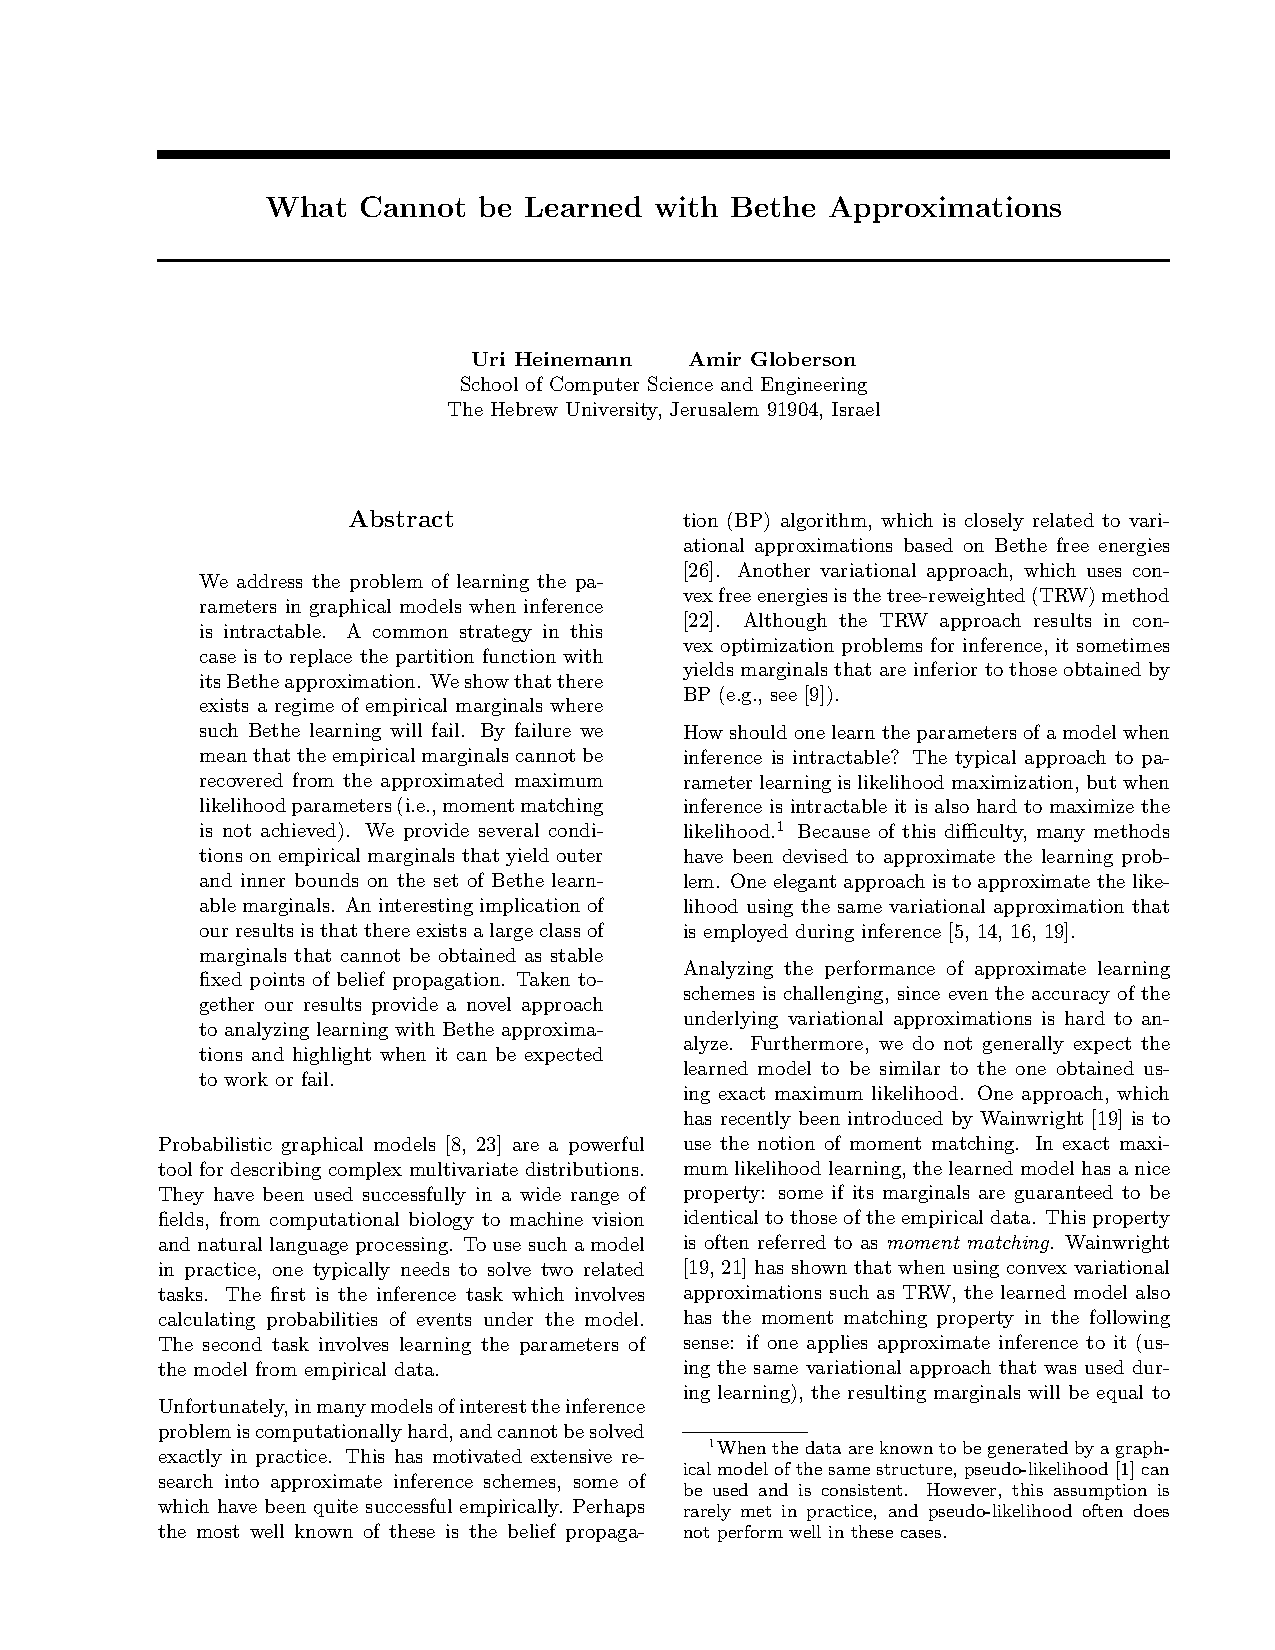
\includepdf[pages=-,pagecommand=\thispagestyle{plain}]{papers/lwb.pdf}}

%%%%%%%%%%%%%%%%%%%%%%%%%%%%%%%%%%%%%%
\newpage
\section{Inferning with high girth graphical models}
\label{sec:lg}
\includepapers{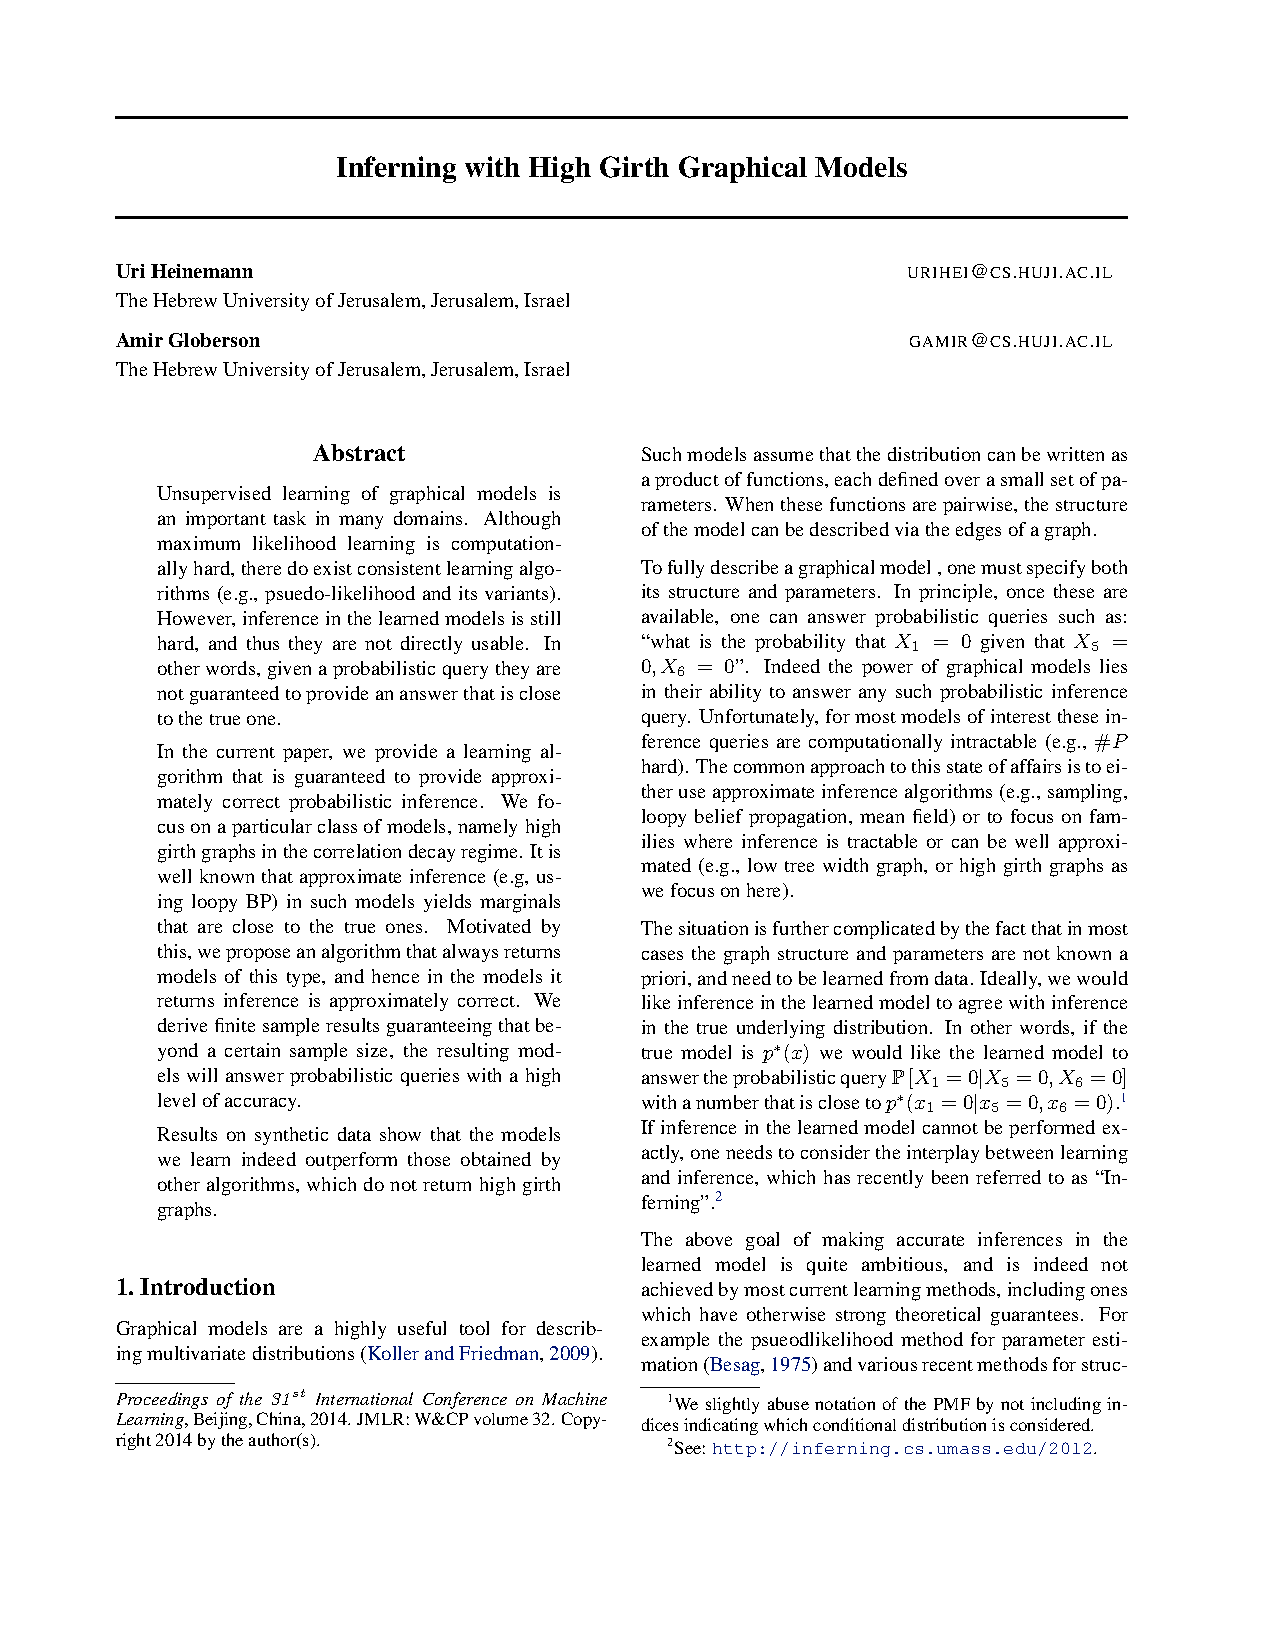
\includepdf[pages=-,pagecommand=\thispagestyle{plain}]{papers/lg.pdf}}
\includepapers{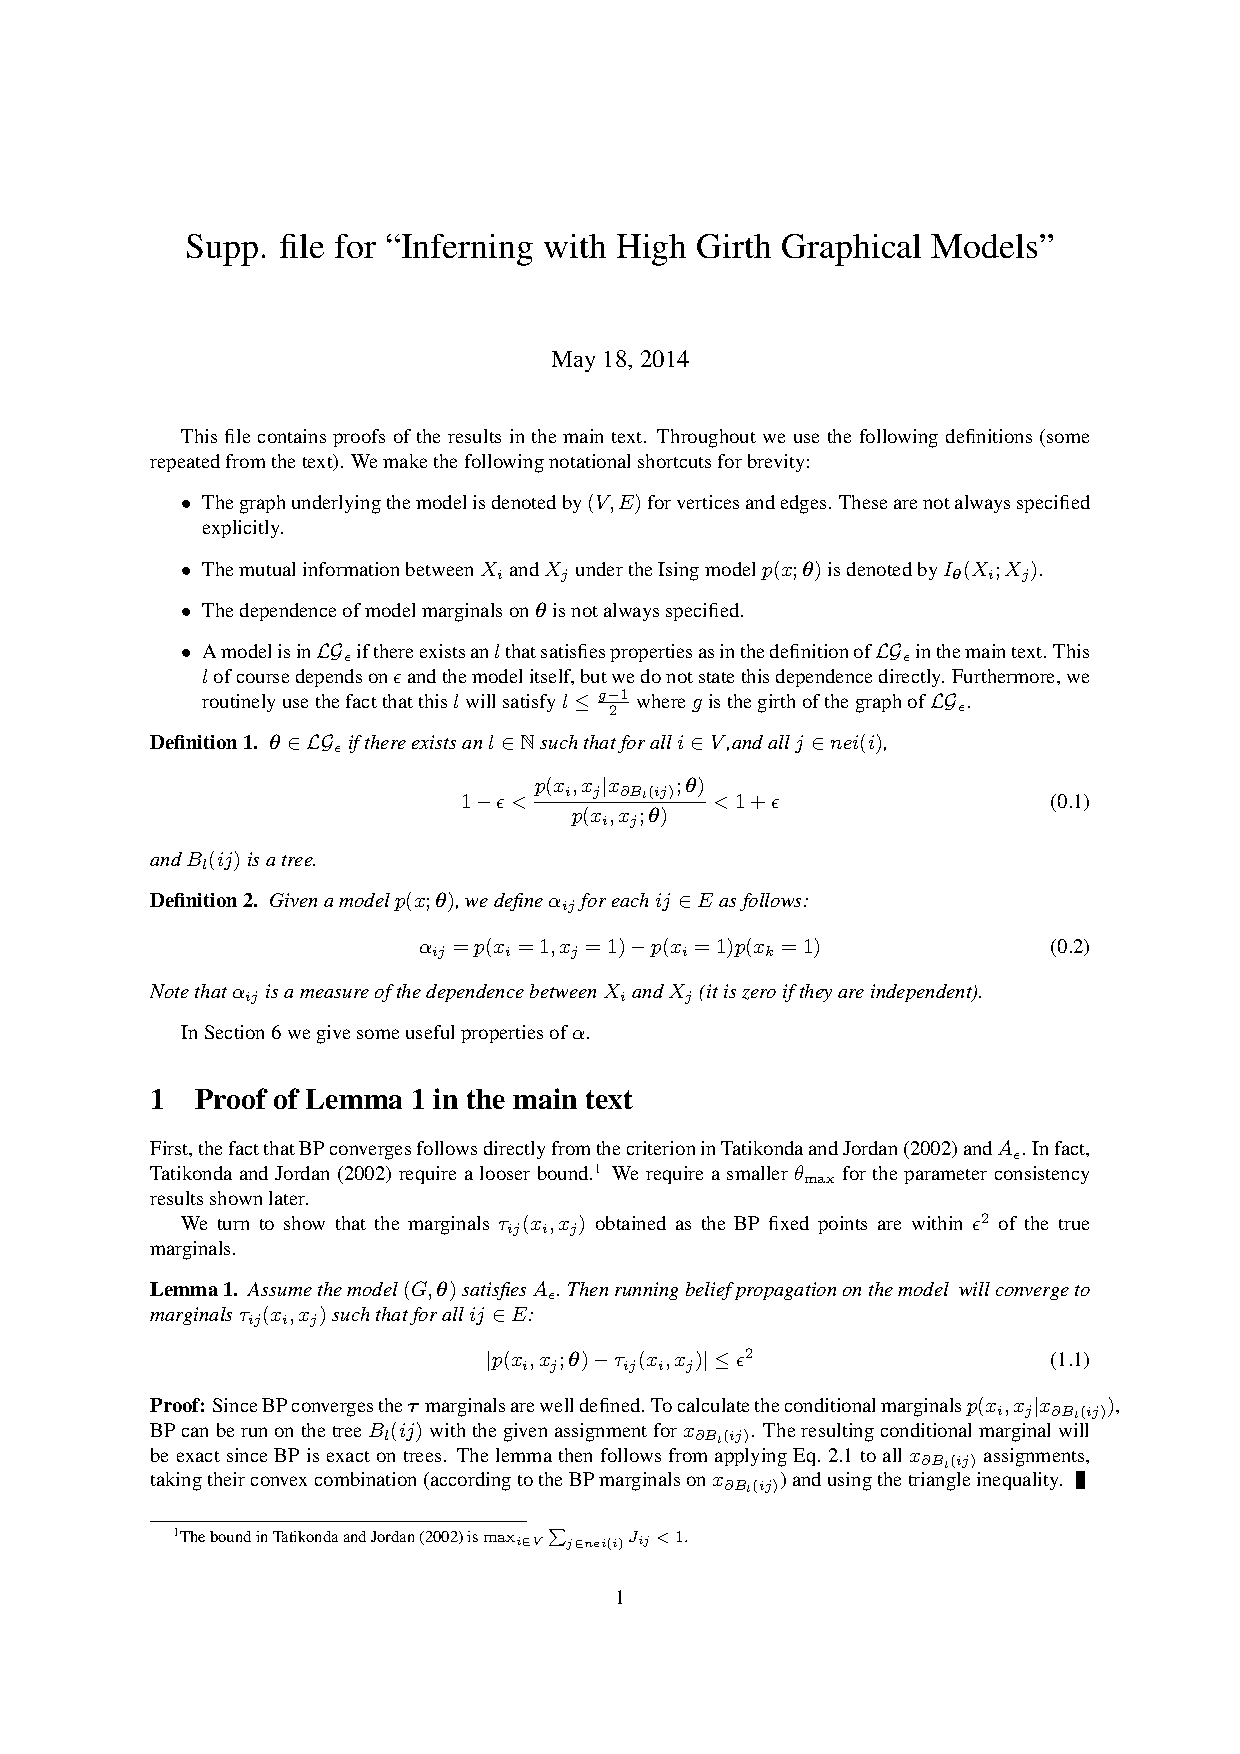
\includepdf[pages=-,pagecommand=\thispagestyle{plain}]{papers/lg_sup.pdf}}

%%%%%%%%%%%%%%%%%%%%%%%%%%%%%%%%%%%%%%
\newpage
\section{Improper Deep Kernels}
\label{sec:impnet}
\includepapers{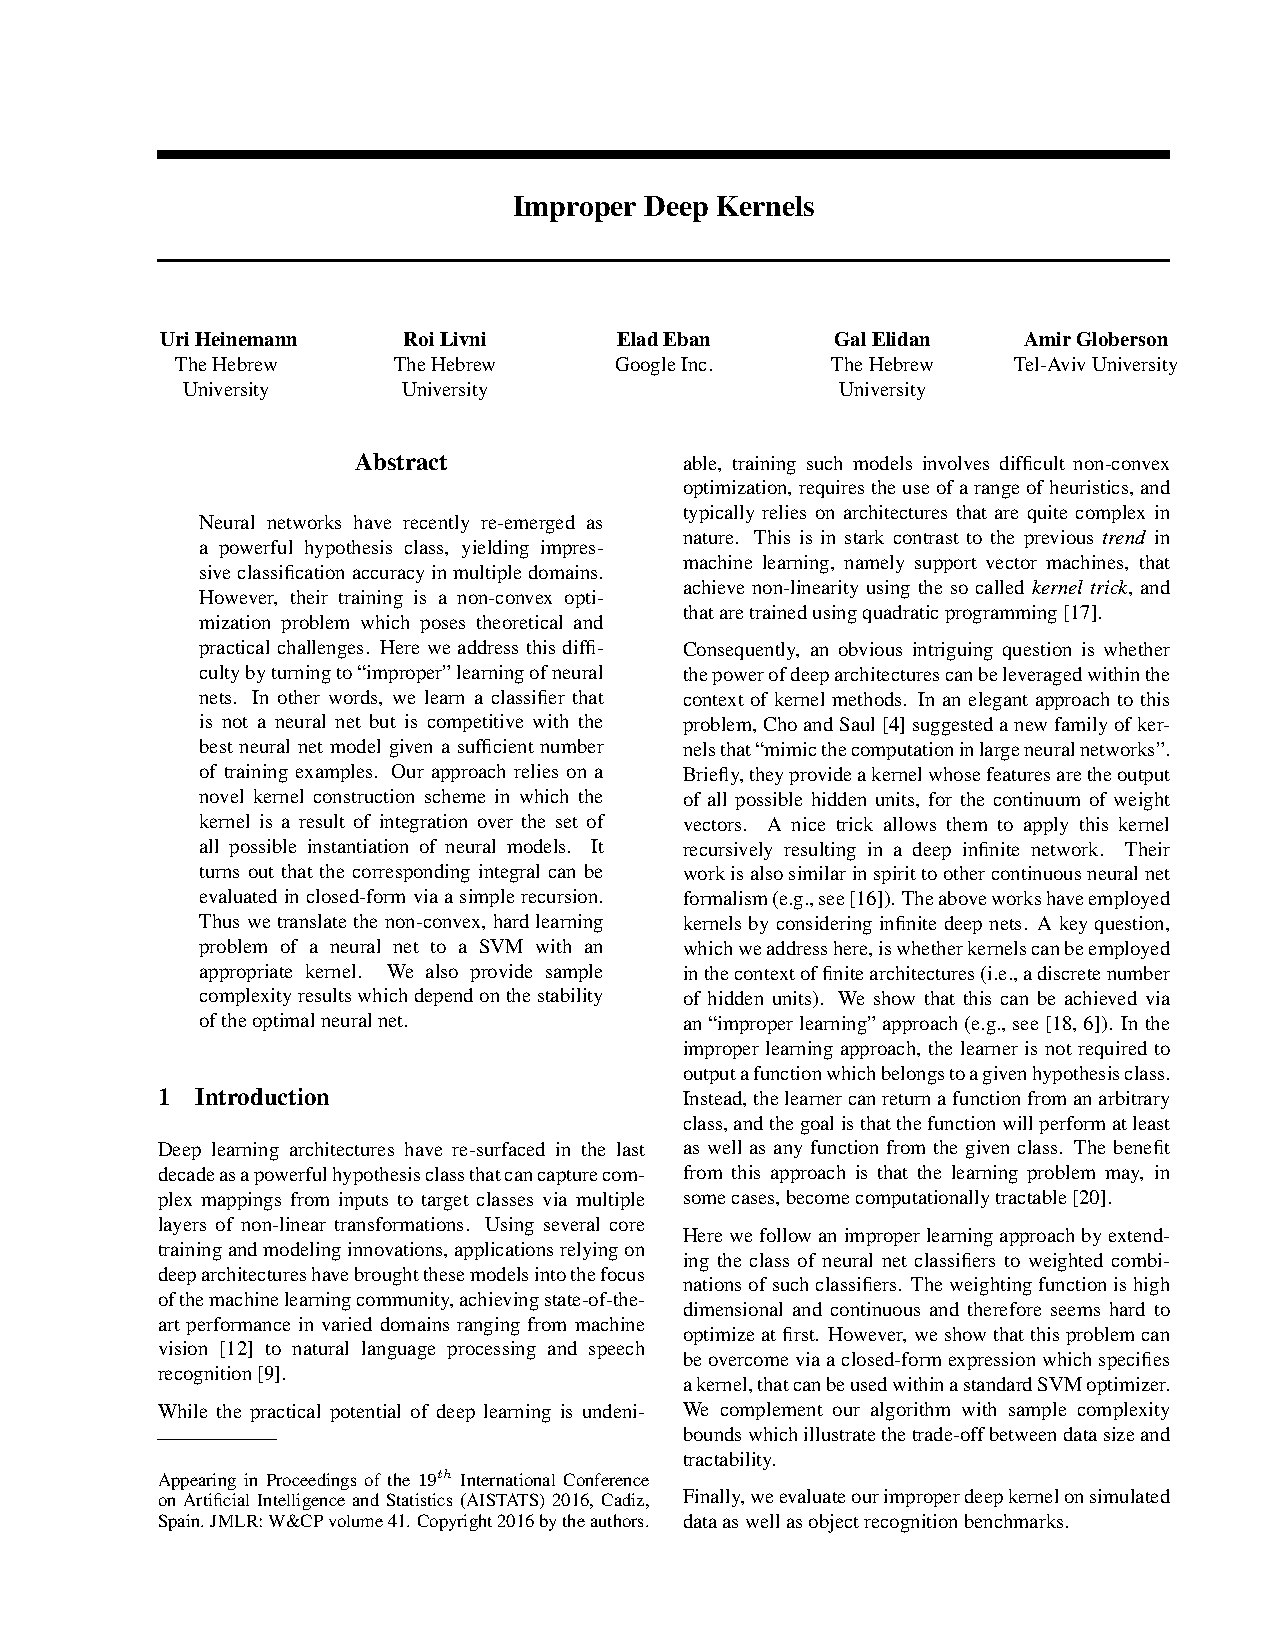
\includepdf[pages=-,pagecommand=\thispagestyle{plain}]{papers/impnet.pdf}}

